\documentclass{article}
\usepackage[T1]{fontenc}
\usepackage[ansinew ]{inputenc}
\usepackage{amsmath}
\usepackage{tikz}
\usepackage{tikzsymbols}
\usepackage{lmodern}
\usepackage{xcolor}
\usetikzlibrary{arrows,automata}
\setlength\parindent{0pt}

\begin{document}

\begin{center}
  \Large{Informatik D - �bungsblatt 3}

  \large{Sebastian H�ffner, Andrea Suckro}
\end{center}



\section{Aufgabe 3.1}
Sei $L \subseteq \Sigma^{*}$ eine endliche Sprache, d.h. eine Sprache mit endlicher Anzahl W�rtern $\omega \in L$ endlicher L�nge. Dann k�nnen wir eine Grammatik definieren, die individuell alle W�rter aus $L$ generiert.
\begin{align*}
S\ \rightarrow\ \omega_i\ |\ \omega_{i+1}\ |\ ...
\end{align*}
Diese Grammatik kann in eine regul�re Grammatik �berf�hrt werden, indem jedes Wort $\omega_i$ als Verkettung von Regeln dargestellt wird.
\begin{align*}
S\ &\rightarrow\ O_{i,0}\ |\ O_{i+1,0}\ |\ ...\\
O_{i,0}\ &\rightarrow\ \omega_{i,0} O_{i,1} \\
O_{i,1}\ &\rightarrow\ \omega_{i,1} O_{i,2} \\
...
\end{align*}
In der Vorlesung wurde bereits gezeigt, dass regul�re Grammatiken in regul�re Ausdr�cke und endliche Automaten �berf�hrt werden k�nnen, also ist die endliche Sprache ebenfalls regul�r.



\section{Aufgabe 3.2}
\subsection{Aufgabe 3.2 (a)}
\begin{align*}
Z_1 &\rightarrow\ 1\ |\ 1Z_2 \\
Z_2 &\rightarrow\ 1\ |\ 1Z_2\ |\ 0Z_3 \\
Z_3 &\rightarrow\ 1\ |\ 0Z_1
%Z_4 &\rightarrow\ 
\end{align*}

\subsection{Aufgabe 3.2 (b)}
\begin{center}
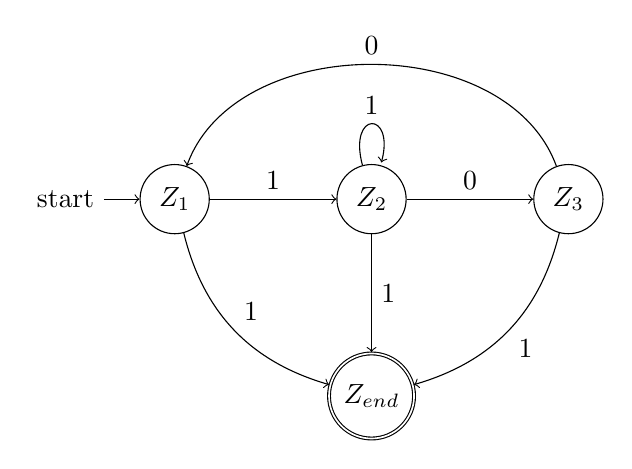
\begin{tikzpicture}[->, auto, node distance=2.5cm]
  \node[initial,state]   (Z1)               {$Z_1$};
  \node[state]           (Z2) [right of=Z1] {$Z_2$};
  \node[state]           (Z3) [right of=Z2] {$Z_3$};
  \node[state,accepting] (Ze) [below of=Z2] {$Z_{end}$};

  \path (Z1) edge [bend right]           node {1} (Ze)
             edge                        node {1} (Z2)
        (Z2) edge                        node {1} (Ze)
             edge [loop above]           node {1} (Z2)
             edge                        node {0} (Z3)
        (Z3) edge [bend left]            node {1} (Ze)
             edge [above, bend right=70] node {0} (Z1)
        ;
\end{tikzpicture}
\end{center}



\section{Aufgabe 3.3}
\begin{center}
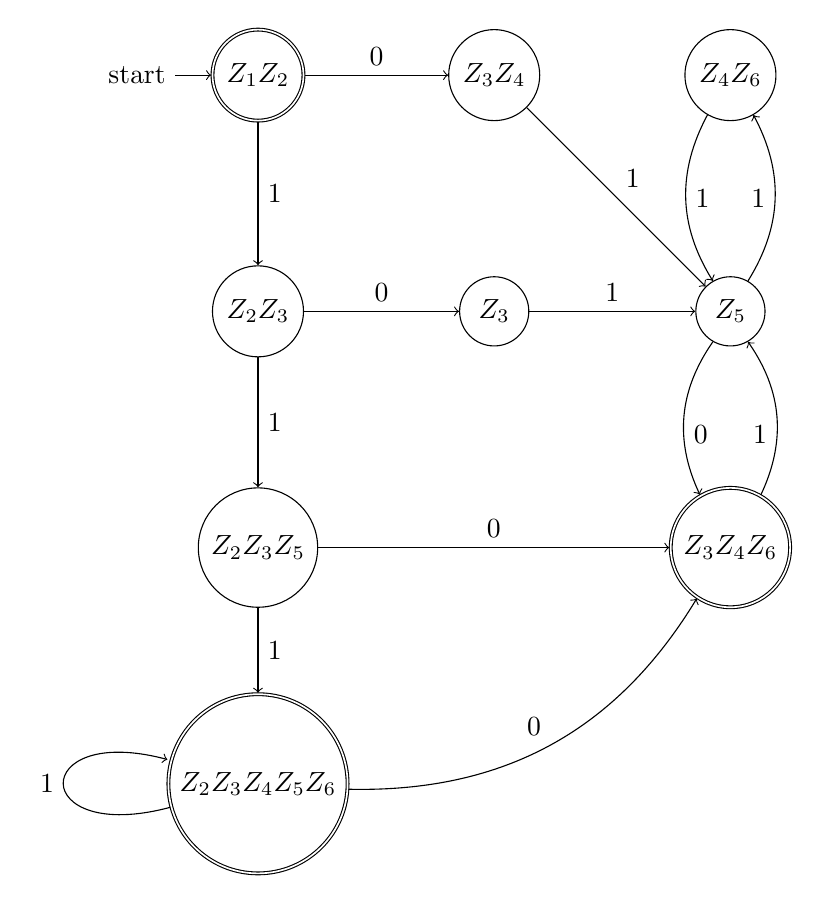
\begin{tikzpicture}[->, auto, node distance=3cm]
  \node[initial,state,accepting] (Z1Z2)                               {$Z_1Z_2$};
  \node[state]                   (Z2Z3)       [below of=Z1Z2]         {$Z_2Z_3$};
  \node[state]                   (Z2Z3Z5)     [below of=Z2Z3]         {$Z_2Z_3Z_5$};
  \node[state,accepting]         (Z2Z3Z4Z5Z6) [below of=Z2Z3Z5]       {$Z_2Z_3Z_4Z_5Z_6$};
  \node[state]                   (Z3)         [right of=Z2Z3]         {$Z_3$};
  \node[state]                   (Z3Z4)       [right of=Z1Z2]         {$Z_3Z_4$};
  \node[state]                   (Z5)         [right of=Z3]           {$Z_5$};
  \node[state]                   (Z4Z6)       [above of=Z5]           {$Z_4Z_6$};
  \node[state,accepting]         (Z3Z4Z6)     [below of=Z5]           {$Z_3Z_4Z_6$};

  \path (Z1Z2)       edge [] node {0} (Z3Z4)
                     edge [] node {1} (Z2Z3)
        (Z2Z3)       edge [] node {0} (Z3)
                     edge [] node {1} (Z2Z3Z5)
        (Z2Z3Z5)     edge [] node {0} (Z3Z4Z6)
                     edge [] node {1} (Z2Z3Z4Z5Z6)
        (Z2Z3Z4Z5Z6) edge [bend right] node {0} (Z3Z4Z6)
                     edge [loop left]  node {1} (Z2Z3Z4Z5Z6)
        (Z3)         %edge [] node {0} ()
                     edge [] node {1} (Z5)
        (Z3Z4)       %edge [] node {0} ()
                     edge [] node {1} (Z5)
        (Z4Z6)       %edge [] node {0} ()
                     edge [bend right] node {1} (Z5)
        (Z5)         edge [bend right] node {0} (Z3Z4Z6)
                     edge [bend right] node {1} (Z4Z6)
        (Z3Z4Z6)     %edge [] node {0} ()
                     edge [bend right] node {1} (Z5)
        ;
\end{tikzpicture}
\end{center}



\section{Aufgabe 3.4}
Wir betrachten zuerst die �u�erste Alternative: $($\colorbox{gray!25}{$(b|a)^*d$}$|$\colorbox{gray!25}{$c$}$)$. Unser NDEA bekommt also je einen $\epsilon$-�bergang zu $(b|a)^*d$ (beginnend bei $Z_2$) und $c$ (beginnend bei $Z_9$). Der Automat zu $c$ ist trivial:

\begin{center}
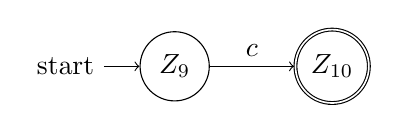
\begin{tikzpicture}[->, auto, node distance=2cm]
  \node[initial,state]   (Z9)                {$Z_9$};
  \node[state,accepting] (Z10) [right of=Z9] {$Z_{10}$};

  \path (Z9) edge node {$c$} (Z10)
        ;
\end{tikzpicture}
\end{center}

Der Teilautomat $(b|a)^*d$ ist etwas komplizierter. Zuerst hat er erneut eine Alternative: $($\colorbox{gray!25}{$b$}$|$\colorbox{gray!25}{$a$}$)$. 
Die Teilautomaten zu $b$ (beginnend bei $Z_3$) und $a$ (beginnend bei $Z_4$) sind wieder trivial:

\begin{center}
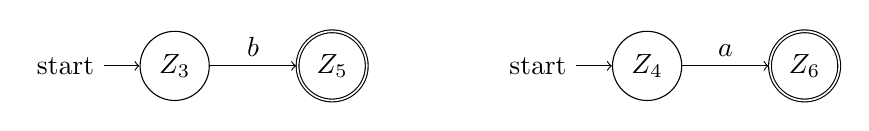
\begin{tikzpicture}[->, auto, node distance=2cm]
  \node[initial,state]   (Z3)               {$Z_3$};
  \node[state,accepting] (Z5) [right of=Z3] {$Z_5$};
  \node[initial,state]   (Z4) [right of=Z5, node distance=4cm] {$Z_4$};
  \node[state,accepting] (Z6) [right of=Z4] {$Z_6$};

  \path (Z3) edge node {$b$} (Z5)
        (Z4) edge node {$a$} (Z6)
        ;
\end{tikzpicture}
\end{center}

Um die Alternative $(b|a)$ darzustellen k�nnen wir diese beiden Teilautomaten mit $\epsilon$-�berg�ngen von Zustand $Z_2$ aus verkn�pfen (dabei �ndern sich die Start\-zu\-st�n\-de):

\begin{center}
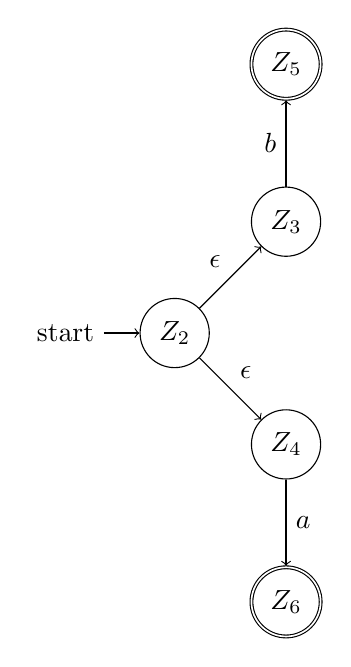
\begin{tikzpicture}[->, auto, node distance=2cm]
  \node[initial,state]   (Z2)                     {$Z_2$};
  \node[state]           (Z3) [above right of=Z2] {$Z_3$};
  \node[state,accepting] (Z5) [above of=Z3]       {$Z_5$};
  \node[state]           (Z4) [below right of=Z2] {$Z_4$};
  \node[state,accepting] (Z6) [below of=Z4]       {$Z_6$};

  \path (Z2) edge node {$\epsilon$} (Z3)
             edge node {$\epsilon$} (Z4)
        (Z3) edge node {$b$}        (Z5)
        (Z4) edge node {$a$}        (Z6)
        ;
\end{tikzpicture}
\end{center}

Als n�chstes k�nnen wir den Kleene-Stern dazu nehmen, um $(a|b)^*$ zu erhalten. Hierzu m�ssen wir den Automaten nur leicht erweitern und die Endzust�nde �ndern:

\begin{center}
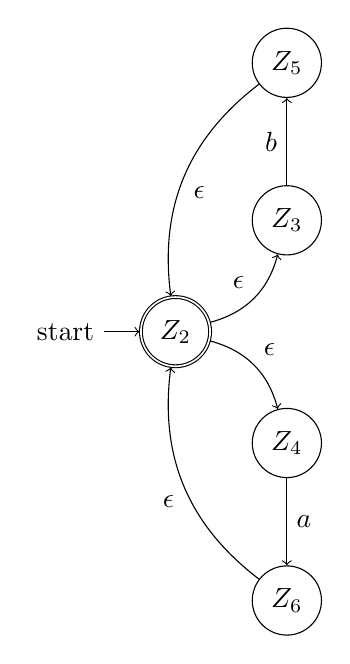
\begin{tikzpicture}[->, auto, node distance=2cm]
  \node[initial,state,accepting] (Z2)                     {$Z_2$};
  \node[state]                   (Z3) [above right of=Z2] {$Z_3$};
  \node[state]                   (Z5) [above of=Z3]       {$Z_5$};
  \node[state]                   (Z4) [below right of=Z2] {$Z_4$};
  \node[state]                   (Z6) [below of=Z4]       {$Z_6$};

  \path (Z2) edge [bend right] node {$\epsilon$} (Z3)
             edge [bend left]  node {$\epsilon$} (Z4)
        (Z3) edge              node {$b$}        (Z5)
        (Z4) edge              node {$a$}        (Z6)
        (Z5) edge [bend right] node {$\epsilon$} (Z2)
        (Z6) edge [bend left]  node {$\epsilon$} (Z2)
        ;
\end{tikzpicture}
\end{center}

Die Verkettung $(a|b)^*d$ folgt als n�chstes. Hierzu muss aus dem Endzustand des aktuellen Automaten ein $\epsilon$-�bergang zu einem weiteren trivialen Automaten, der $d$ akzeptiert, gezogen werden (und erneut der Endzustand verschoben werden).

\begin{center}
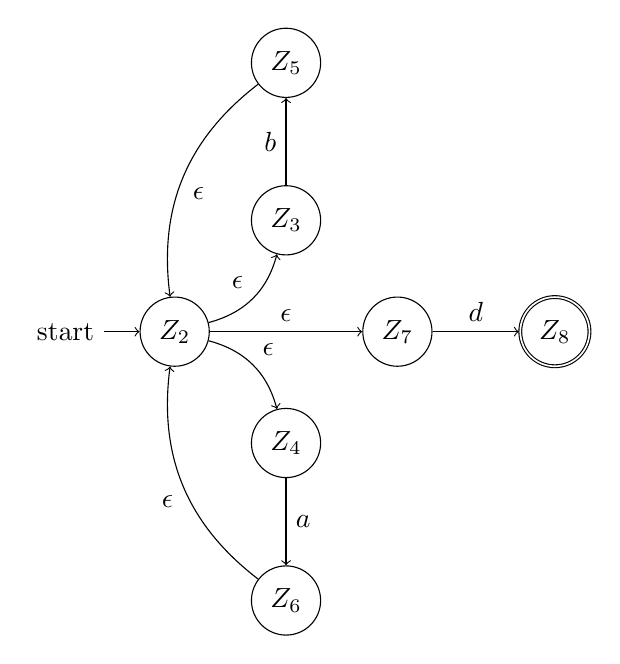
\begin{tikzpicture}[->, auto, node distance=2cm]
  \node[initial,state]   (Z2)                     {$Z_2$};
  \node[state]           (Z3) [above right of=Z2] {$Z_3$};
  \node[state]           (Z5) [above of=Z3]       {$Z_5$};
  \node[state]           (Z4) [below right of=Z2] {$Z_4$};
  \node[state]           (Z6) [below of=Z4]       {$Z_6$};
  \node[state]           (Z7) [below right of=Z3] {$Z_7$};
  \node[state,accepting] (Z8) [right of=Z7]       {$Z_8$};

  \path (Z2) edge [bend right] node {$\epsilon$} (Z3)
             edge [bend left]  node {$\epsilon$} (Z4)
        (Z3) edge              node {$b$}        (Z5)
        (Z4) edge              node {$a$}        (Z6)
        (Z5) edge [bend right] node {$\epsilon$} (Z2)
        (Z6) edge [bend left]  node {$\epsilon$} (Z2)
        (Z2) edge              node {$\epsilon$} (Z7)
        (Z7) edge              node {$d$}        (Z8)
        ;
\end{tikzpicture}
\end{center}

Als letzten Schritt k�nnen wir diesen Automaten und den Automaten vom Beginn ($c$, beginnend mit $Z_9$) erneut mit der Regel f�r Alternativen �ber Zustand $Z_1$ verkn�pfen:

\begin{center}
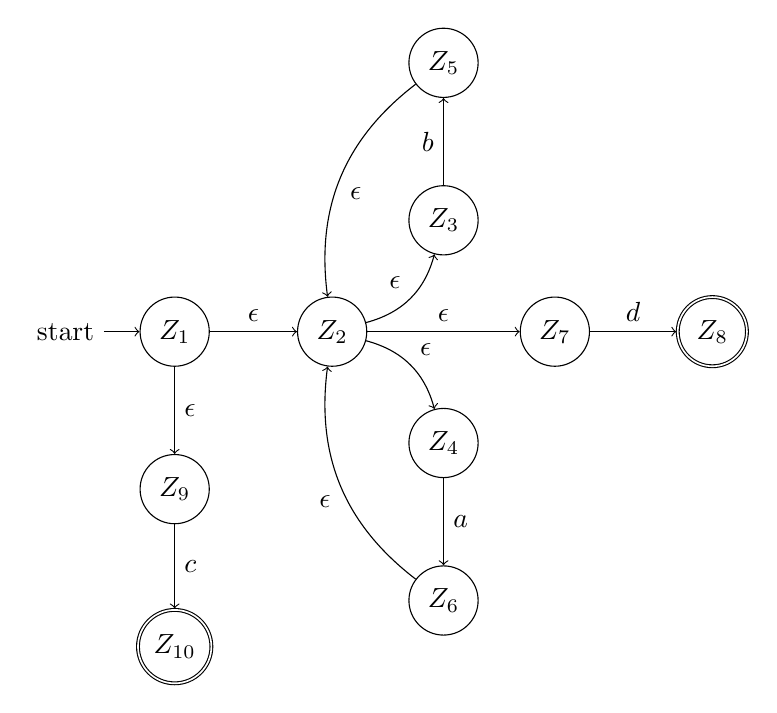
\begin{tikzpicture}[->, auto, node distance=2cm]
  \node[initial,state]   (Z1)                      {$Z_1$};
  \node[state]           (Z2)  [right of=Z1]       {$Z_2$};
  \node[state]           (Z3)  [above right of=Z2] {$Z_3$};
  \node[state]           (Z5)  [above of=Z3]       {$Z_5$};
  \node[state]           (Z4)  [below right of=Z2] {$Z_4$};
  \node[state]           (Z6)  [below of=Z4]       {$Z_6$};
  \node[state]           (Z7)  [below right of=Z3] {$Z_7$};
  \node[state,accepting] (Z8)  [right of=Z7]       {$Z_8$};
  \node[state]           (Z9)  [below of=Z1]       {$Z_9$};
  \node[state,accepting] (Z10) [below of=Z9]       {$Z_{10}$};

  \path (Z1) edge              node {$\epsilon$} (Z2)
        (Z1) edge              node {$\epsilon$} (Z9)
        (Z2) edge [bend right] node {$\epsilon$} (Z3)
             edge [bend left]  node {$\epsilon$} (Z4)
        (Z3) edge              node {$b$}        (Z5)
        (Z4) edge              node {$a$}        (Z6)
        (Z5) edge [bend right] node {$\epsilon$} (Z2)
        (Z6) edge [bend left]  node {$\epsilon$} (Z2)
        (Z2) edge              node {$\epsilon$} (Z7)
        (Z7) edge              node {$d$}        (Z8)
        (Z9) edge              node {$c$}        (Z10)
        ;
\end{tikzpicture}
\end{center}



\section{Aufgabe 3.5}
%\begin{figure}[h]
%  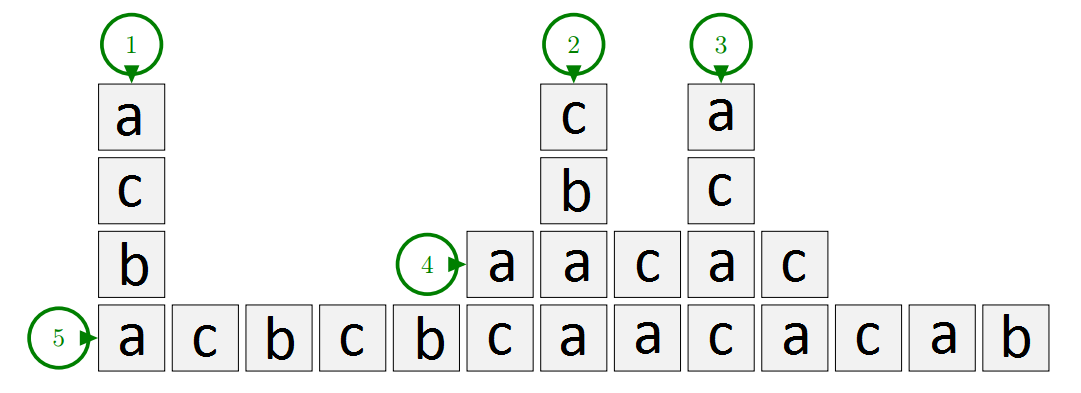
\includegraphics[width=\textwidth]{crossword.png}
%\end{figure}
\begin{enumerate}
	\item bbbbb
  \item bcbca
  \item bdda
  \item adadc
  \item bbaadd
\end{enumerate}



\section{Aufgabe 3.6}
\subsection*{Hilfssubstitutionen und -funktionen}
\begin{align*}
x:&=\epsilon|a|b \\
&\\
aa^* &= a+ \\
a|b+a &= b^*a \\
a|b &= b|a \\
a|aa^*a &= a+ \\
a|ab^* &= ab^*\\
a|ab^*b &= a|ab+ = ab^*\\
\epsilon|a+ &= a*\\
xx^* &= x^* \mbox{ ($\epsilon \in x$)} \\
x+ &= x^* \mbox{ ($\epsilon \in x$)}
\end{align*}


\subsection*{k=0}
\begin{align*}
\alpha^0_{1,1} &= \epsilon \\
\alpha^0_{1,2} &= b \\
\alpha^0_{1,3} &= a \\
\alpha^0_{1,4} &= \emptyset \\
\alpha^0_{2,1} &= \emptyset \\
\alpha^0_{2,2} &= \epsilon \\
\alpha^0_{2,3} &= \emptyset \\
\alpha^0_{2,4} &= \emptyset \\
\alpha^0_{3,1} &= \emptyset \\
\alpha^0_{3,2} &= \emptyset \\
\alpha^0_{3,3} &= \epsilon|a|b = x\\
\alpha^0_{3,4} &= c \\
\alpha^0_{4,1} &= a\\
\alpha^0_{4,2} &= \emptyset \\
\alpha^0_{4,3} &= \emptyset \\
\alpha^0_{4,4} &= \epsilon
\end{align*}

\begin{center}
\begin{tabular}{c||*{3}{c|}c}
$\delta$ & 1 & 2 & 3 & 4 \\
  \hline \hline
1 & $\epsilon$  & $b$         & $a$         & $\emptyset$ \\ \hline
2 & $\emptyset$ & $\epsilon$  & $\emptyset$ & $\emptyset$ \\ \hline
3 & $\emptyset$ & $\emptyset$ & $x$         & $c$         \\ \hline
4 & $a$         & $\emptyset$ & $\emptyset$ & $\epsilon$  \\
\end{tabular}
\end{center}

\subsection*{k=1}
\begin{align*}
\alpha^1_{1,1} &= \left(\alpha^0_{1,1}|\alpha^0_{1,1}\left(\alpha^0_{1,1}\right)^*\alpha^0_{1,1}\right) = \left(\epsilon|\epsilon\left(\epsilon\right)^*\epsilon\right) = \epsilon \\
\alpha^1_{1,2} &= \left(\alpha^0_{1,2}|\alpha^0_{1,1}\left(\alpha^0_{1,1}\right)^*\alpha^0_{1,2}\right) = \left(b|\epsilon\left(\epsilon\right)^*b\right) = b \\
\alpha^1_{1,3} &= \left(\alpha^0_{1,3}|\alpha^0_{1,1}\left(\alpha^0_{1,1}\right)^*\alpha^0_{1,3}\right) = \left(a|\epsilon\left(\epsilon\right)^*a\right) = a \\
\alpha^1_{1,4} &= \left(\alpha^0_{1,4}|\alpha^0_{1,1}\left(\alpha^0_{1,1}\right)^*\alpha^0_{1,4}\right) = \left(\emptyset|\epsilon\left(\epsilon\right)^*\emptyset\right) = \emptyset \\
\alpha^1_{2,1} &= \left(\alpha^0_{2,1}|\alpha^0_{2,1}\left(\alpha^0_{1,1}\right)^*\alpha^0_{1,1}\right) = \left(\emptyset|\emptyset\left(\epsilon\right)^*\epsilon\right) = \emptyset \\
\alpha^1_{2,2} &= \left(\alpha^0_{2,2}|\alpha^0_{2,1}\left(\alpha^0_{1,1}\right)^*\alpha^0_{1,2}\right) = \left(\epsilon|\emptyset\left(\epsilon\right)^*b\right) = \epsilon \\
\alpha^1_{2,3} &= \left(\alpha^0_{2,3}|\alpha^0_{2,1}\left(\alpha^0_{1,1}\right)^*\alpha^0_{1,3}\right) = \left(\emptyset|\emptyset\left(\epsilon\right)^*a\right) = \emptyset \\
\alpha^1_{2,4} &= \left(\alpha^0_{2,4}|\alpha^0_{2,1}\left(\alpha^0_{1,1}\right)^*\alpha^0_{1,4}\right) = \left(\emptyset|\emptyset\left(\epsilon\right)^*\emptyset\right) = \emptyset \\
\alpha^1_{3,1} &= \left(\alpha^0_{3,1}|\alpha^0_{3,1}\left(\alpha^0_{1,1}\right)^*\alpha^0_{1,1}\right) = \left(\emptyset|\emptyset\left(\epsilon\right)^*\epsilon\right) = \emptyset \\
\alpha^1_{3,2} &= \left(\alpha^0_{3,2}|\alpha^0_{3,1}\left(\alpha^0_{1,1}\right)^*\alpha^0_{1,2}\right) = \left(\emptyset|\emptyset\left(\epsilon\right)^*b\right) = \emptyset \\
\alpha^1_{3,3} &= \left(\alpha^0_{3,3}|\alpha^0_{3,1}\left(\alpha^0_{1,1}\right)^*\alpha^0_{1,3}\right) = \left(x|\emptyset\left(\epsilon\right)^*a\right) = x \\
\alpha^1_{3,4} &= \left(\alpha^0_{3,4}|\alpha^0_{3,1}\left(\alpha^0_{1,1}\right)^*\alpha^0_{1,4}\right) = \left(c|\emptyset\left(\epsilon\right)^*\emptyset\right) = c \\
\alpha^1_{4,1} &= \left(\alpha^0_{4,1}|\alpha^0_{4,1}\left(\alpha^0_{1,1}\right)^*\alpha^0_{1,1}\right) = \left(a|a\left(\epsilon\right)^*\epsilon\right) = a \\
\alpha^1_{4,2} &= \left(\alpha^0_{4,2}|\alpha^0_{4,1}\left(\alpha^0_{1,1}\right)^*\alpha^0_{1,2}\right) = \left(\emptyset|a\left(\epsilon\right)^*b\right) = ab \\
\alpha^1_{4,3} &= \left(\alpha^0_{4,3}|\alpha^0_{4,1}\left(\alpha^0_{1,1}\right)^*\alpha^0_{1,3}\right) = \left(\emptyset|a\left(\epsilon\right)^*a\right) = aa \\
\alpha^1_{4,4} &= \left(\alpha^0_{4,4}|\alpha^0_{4,1}\left(\alpha^0_{1,1}\right)^*\alpha^0_{1,4}\right) = \left(\epsilon|a\left(\epsilon\right)^*\emptyset\right) = \epsilon 
\end{align*}

\begin{center}
\begin{tabular}{c||*{3}{c|}c}
$\delta$ & 1 & 2 & 3 & 4 \\
  \hline \hline
1 & $\epsilon$  & $b$         & $a$         & $\emptyset$ \\ \hline
2 & $\emptyset$ & $\epsilon$  & $\emptyset$ & $\emptyset$ \\ \hline
3 & $\emptyset$ & $\emptyset$ & $x$         & $c$         \\ \hline
4 & $a$         & $ab$        & $aa$        & $\epsilon$  \\
\end{tabular}
\end{center}

\subsection*{k=2}
\begin{align*}
\alpha^2_{1,1} &= \left(\alpha^1_{1,1}|\alpha^1_{1,2}\left(\alpha^1_{2,2}\right)^*\alpha^1_{2,1}\right) = \left(\epsilon|b\left(\epsilon\right)^*\emptyset\right) = \epsilon \\
\alpha^2_{1,2} &= \left(\alpha^1_{1,2}|\alpha^1_{1,2}\left(\alpha^1_{2,2}\right)^*\alpha^1_{2,2}\right) = \left(b|b\left(\epsilon\right)^*\epsilon\right) = b \\
\alpha^2_{1,3} &= \left(\alpha^1_{1,3}|\alpha^1_{1,2}\left(\alpha^1_{2,2}\right)^*\alpha^1_{2,3}\right) = \left(a|b\left(\epsilon\right)^*\emptyset\right) = a \\
\alpha^2_{1,4} &= \left(\alpha^1_{1,4}|\alpha^1_{1,2}\left(\alpha^1_{2,2}\right)^*\alpha^1_{2,4}\right) = \left(\emptyset|b\left(\epsilon\right)^*\emptyset\right) = \emptyset \\
\alpha^2_{2,1} &= \left(\alpha^1_{2,1}|\alpha^1_{2,2}\left(\alpha^1_{2,2}\right)^*\alpha^1_{2,1}\right) = \left(\emptyset|\epsilon\left(\epsilon\right)^*\emptyset\right) = \emptyset \\
\alpha^2_{2,2} &= \left(\alpha^1_{2,2}|\alpha^1_{2,2}\left(\alpha^1_{2,2}\right)^*\alpha^1_{2,2}\right) = \left(\epsilon|\epsilon\left(\epsilon\right)^*\epsilon\right) = \epsilon \\
\alpha^2_{2,3} &= \left(\alpha^1_{2,3}|\alpha^1_{2,2}\left(\alpha^1_{2,2}\right)^*\alpha^1_{2,3}\right) = \left(\emptyset|\epsilon\left(\epsilon\right)^*\emptyset\right) = \emptyset \\
\alpha^2_{2,4} &= \left(\alpha^1_{2,4}|\alpha^1_{2,2}\left(\alpha^1_{2,2}\right)^*\alpha^1_{2,4}\right) = \left(\emptyset|\epsilon\left(\epsilon\right)^*\emptyset\right) = \emptyset \\
\alpha^2_{3,1} &= \left(\alpha^1_{3,1}|\alpha^1_{3,2}\left(\alpha^1_{2,2}\right)^*\alpha^1_{2,1}\right) = \left(\emptyset|\emptyset\left(\epsilon\right)^*\emptyset\right) = \emptyset \\
\alpha^2_{3,2} &= \left(\alpha^1_{3,2}|\alpha^1_{3,2}\left(\alpha^1_{2,2}\right)^*\alpha^1_{2,2}\right) = \left(\emptyset|\emptyset\left(\epsilon\right)^*\epsilon\right) = \emptyset \\
\alpha^2_{3,3} &= \left(\alpha^1_{3,3}|\alpha^1_{3,2}\left(\alpha^1_{2,2}\right)^*\alpha^1_{2,3}\right) = \left(x|\emptyset\left(\epsilon\right)^*\emptyset\right) = x \\
\alpha^2_{3,4} &= \left(\alpha^1_{3,4}|\alpha^1_{3,2}\left(\alpha^1_{2,2}\right)^*\alpha^1_{2,4}\right) = \left(c|\emptyset\left(\epsilon\right)^*\emptyset\right) = c \\
\alpha^2_{4,1} &= \left(\alpha^1_{4,1}|\alpha^1_{4,2}\left(\alpha^1_{2,2}\right)^*\alpha^1_{2,1}\right) = \left(a|ab\left(\epsilon\right)^*\emptyset\right) = a \\
\alpha^2_{4,2} &= \left(\alpha^1_{4,2}|\alpha^1_{4,2}\left(\alpha^1_{2,2}\right)^*\alpha^1_{2,2}\right) = \left(ab|ab\left(\epsilon\right)^*\epsilon\right) = ab \\
\alpha^2_{4,3} &= \left(\alpha^1_{4,3}|\alpha^1_{4,2}\left(\alpha^1_{2,2}\right)^*\alpha^1_{2,3}\right) = \left(aa|ab\left(\epsilon\right)^*\emptyset\right) = aa \\
\alpha^2_{4,4} &= \left(\alpha^1_{4,4}|\alpha^1_{4,2}\left(\alpha^1_{2,2}\right)^*\alpha^1_{2,4}\right) = \left(\epsilon|ab\left(\epsilon\right)^*\emptyset\right) = \epsilon
\end{align*}

\begin{center}
\begin{tabular}{c||*{3}{c|}c}
$\delta$ & 1 & 2 & 3 & 4 \\
  \hline \hline
1 & $\epsilon$  & $b$         & $a$         & $\emptyset$ \\ \hline
2 & $\emptyset$ & $\epsilon$  & $\emptyset$ & $\emptyset$ \\ \hline
3 & $\emptyset$ & $\emptyset$ & $x$         & $c$         \\ \hline
4 & $a$         & $ab$        & $aa$        & $\epsilon$  \\
\end{tabular}
\end{center}

\subsection*{k=3}
\begin{align*}
\alpha^3_{1,1} &= \left(\alpha^2_{1,1}|\alpha^2_{1,3}\left(\alpha^2_{3,3}\right)^*\alpha^2_{3,1}\right) = \left(\epsilon|a\left(x\right)^*\emptyset\right) = \epsilon \\
\alpha^3_{1,2} &= \left(\alpha^2_{1,2}|\alpha^2_{1,3}\left(\alpha^2_{3,3}\right)^*\alpha^2_{3,2}\right) = \left(b|a\left(x\right)^*\emptyset\right) = b \\
\alpha^3_{1,3} &= \left(\alpha^2_{1,3}|\alpha^2_{1,3}\left(\alpha^2_{3,3}\right)^*\alpha^2_{3,3}\right) = \left(a|a\left(x\right)^*x\right) = a|ax^*x = a|ax+ = ax^*\\
\alpha^3_{1,4} &= \left(\alpha^2_{1,4}|\alpha^2_{1,3}\left(\alpha^2_{3,3}\right)^*\alpha^2_{3,4}\right) = \left(\emptyset|a\left(x\right)^*c\right) = ax^*c\\
\alpha^3_{2,1} &= \left(\alpha^2_{2,1}|\alpha^2_{2,3}\left(\alpha^2_{3,3}\right)^*\alpha^2_{3,1}\right) = \left(\emptyset|\emptyset\left(x\right)^*\emptyset\right) = \emptyset \\
\alpha^3_{2,2} &= \left(\alpha^2_{2,2}|\alpha^2_{2,3}\left(\alpha^2_{3,3}\right)^*\alpha^2_{3,2}\right) = \left(\epsilon|\emptyset\left(x\right)^*\emptyset\right) = \epsilon \\
\alpha^3_{2,3} &= \left(\alpha^2_{2,3}|\alpha^2_{2,3}\left(\alpha^2_{3,3}\right)^*\alpha^2_{3,3}\right) = \left(\emptyset|\emptyset\left(x\right)^*x\right) = \emptyset \\
\alpha^3_{2,4} &= \left(\alpha^2_{2,4}|\alpha^2_{2,3}\left(\alpha^2_{3,3}\right)^*\alpha^2_{3,4}\right) = \left(\emptyset|\emptyset\left(x\right)^*c\right) = \emptyset \\
\alpha^3_{3,1} &= \left(\alpha^2_{3,1}|\alpha^2_{3,3}\left(\alpha^2_{3,3}\right)^*\alpha^2_{3,1}\right) = \left(\emptyset|x\left(x\right)^*\emptyset\right) = \emptyset \\
\alpha^3_{3,2} &= \left(\alpha^2_{3,2}|\alpha^2_{3,3}\left(\alpha^2_{3,3}\right)^*\alpha^2_{3,2}\right) = \left(\emptyset|x\left(x\right)^*\emptyset\right) = \emptyset \\
\alpha^3_{3,3} &= \left(\alpha^2_{3,3}|\alpha^2_{3,3}\left(\alpha^2_{3,3}\right)^*\alpha^2_{3,3}\right) = \left(x|x\left(x\right)^*x\right) = x|xx^*x = x|xx+ = x+ \\
\alpha^3_{3,4} &= \left(\alpha^2_{3,4}|\alpha^2_{3,3}\left(\alpha^2_{3,3}\right)^*\alpha^2_{3,4}\right) = \left(c|x\left(x\right)^*c\right) = c|xx^*c = c|x+c = x^*c \\
\alpha^3_{4,1} &= \left(\alpha^2_{4,1}|\alpha^2_{4,3}\left(\alpha^2_{3,3}\right)^*\alpha^2_{3,1}\right) = \left(a|aa\left(x\right)^*\emptyset\right) = a \\
\alpha^3_{4,2} &= \left(\alpha^2_{4,2}|\alpha^2_{4,3}\left(\alpha^2_{3,3}\right)^*\alpha^2_{3,2}\right) = \left(ab|aa\left(x\right)^*\emptyset\right) = ab \\
\alpha^3_{4,3} &= \left(\alpha^2_{4,3}|\alpha^2_{4,3}\left(\alpha^2_{3,3}\right)^*\alpha^2_{3,3}\right) = \left(aa|aa\left(x\right)^*x\right) = aa|aax^*x = aax^* \\
\alpha^3_{4,4} &= \left(\alpha^2_{4,4}|\alpha^2_{4,3}\left(\alpha^2_{3,3}\right)^*\alpha^2_{3,4}\right) = \left(\epsilon|aa\left(x\right)^*c\right) = \epsilon|aax^*c
\end{align*}

\begin{center}
\begin{tabular}{c||*{3}{c|}c}
$\delta$ & 1 & 2 & 3 & 4 \\
  \hline \hline
1 & $\epsilon$  & $b$         & $a|ax^*x$   & $ax^*c$            \\ \hline
2 & $\emptyset$ & $\epsilon$  & $\emptyset$ & $\emptyset$        \\ \hline
3 & $\emptyset$ & $\emptyset$ & $x|xx^*x$   & $c|xx^*c$          \\ \hline
4 & $a$         & $ab$        & $aa|aax^*x$ & $\epsilon|aax^*c$  \\
\end{tabular}

\begin{tabular}{c||*{3}{c|}c}
$\delta$ & 1 & 2 & 3 & 4 \\
  \hline \hline
1 & $\epsilon$  & $b$         & $ax^*$      & $ax^*c$            \\ \hline
2 & $\emptyset$ & $\epsilon$  & $\emptyset$ & $\emptyset$        \\ \hline
3 & $\emptyset$ & $\emptyset$ & $x+$        & $x^*c$             \\ \hline
4 & $a$         & $ab$        & $aax^*$     & $\epsilon|aax^*c$  \\
\end{tabular}
\end{center}

\subsection*{k=4}
\begin{align*}
\alpha^4_{1,1} &= \left(\alpha^3_{1,1}|\alpha^3_{1,4}\left(\alpha^3_{4,4}\right)^*\alpha^3_{4,1}\right) \\&= \left(\epsilon|ax^*c\left(\epsilon|aax^*c\right)^*a\right) = \left(\epsilon|ax^*c\left(aax^*c\right)^*a\right) = \left(\epsilon|\left(ax^*ca\right)+\right) = \left(ax^*ca\right)^*\\
\alpha^4_{1,2} &= \left(\alpha^3_{1,2}|\alpha^3_{1,4}\left(\alpha^3_{4,4}\right)^*\alpha^3_{4,2}\right) \\&= \left(b|ax^*c\left(\epsilon|aax^*c\right)^*ab\right) = \left(b|ax^*c\left(aax^*c\right)^*ab\right) = \left(b|\left(ax^*ca\right)+b\right) \\&= \left(ax^*ca\right)^*b \\
\alpha^4_{1,3} &= \left(\alpha^3_{1,3}|\alpha^3_{1,4}\left(\alpha^3_{4,4}\right)^*\alpha^3_{4,3}\right) \\&= \left(\left(a|ax^*x\right)|ax^*c\left(\epsilon|aax^*c\right)^*\left(aa|aax^*x\right)\right) \\&= \left(ax^*|ax^*c\left(\epsilon|aax^*c\right)^*\left(aa|aax^*x\right)\right) = \left(ax^*|ax^*c\left(\epsilon|aax^*c\right)^*aax^*\right) \\&= \left(ax^*|(ax^*ca)+ax^*\right) = (ax^*ca)^*ax^*\\
\alpha^4_{1,4} &= \left(\alpha^3_{1,4}|\alpha^3_{1,4}\left(\alpha^3_{4,4}\right)^*\alpha^3_{4,4}\right) \\&= \left(ax^*c|ax^*c\left(\epsilon|aax^*c\right)^*\left(\epsilon|aax^*c\right)\right) = \left(ax^*c|ax^*c\left(aax^*c\right)^*aax^*c\right) \\&= \left(ax^*c|\left(ax^*ca\right)+ax^*c\right) = \left(ax^*ca\right)^*ax^*c \\
\alpha^4_{2,1} &= \left(\alpha^3_{2,1}|\alpha^3_{2,4}\left(\alpha^3_{4,4}\right)^*\alpha^3_{4,1}\right) = \left(\emptyset|\emptyset\left(\epsilon|aax^*c\right)^*a\right) = \emptyset \\
\alpha^4_{2,2} &= \left(\alpha^3_{2,2}|\alpha^3_{2,4}\left(\alpha^3_{4,4}\right)^*\alpha^3_{4,2}\right) = \left(\epsilon|\emptyset\left(\epsilon|aax^*c\right)^*ab\right) = \epsilon \\
\alpha^4_{2,3} &= \left(\alpha^3_{2,3}|\alpha^3_{2,4}\left(\alpha^3_{4,4}\right)^*\alpha^3_{4,3}\right) = \left(\emptyset|\emptyset\left(\epsilon|aax^*c\right)^*\left(aa|aax^*x\right)\right) = \emptyset \\
\alpha^4_{2,4} &= \left(\alpha^3_{2,4}|\alpha^3_{2,4}\left(\alpha^3_{4,4}\right)^*\alpha^3_{4,4}\right) = \left(\emptyset|\emptyset\left(\epsilon|aax^*c\right)^*\left(\epsilon|aax^*c\right)\right) = \emptyset
\end{align*}

\begin{align*}
\alpha^4_{3,1} &= \left(\alpha^3_{3,1}|\alpha^3_{3,4}\left(\alpha^3_{4,4}\right)^*\alpha^3_{4,1}\right) \\&= \left(\emptyset|\left(c|xx^*c\right)\left(\epsilon|aax^*c\right)^*a\right) = \left(c|xx^*c\right)\left(\epsilon|aax^*c\right)^*a = \left(c|xx^*c\right)\left(aax^*c\right)^*a \\&= x^*c\left(aax^*c\right)^*a = \left(x^*caa\right)^*x^*ca \\
\alpha^4_{3,2} &= \left(\alpha^3_{3,2}|\alpha^3_{3,4}\left(\alpha^3_{4,4}\right)^*\alpha^3_{4,2}\right) \\&= \left(\emptyset|\left(c|xx^*c\right)\left(\epsilon|aax^*c\right)^*ab\right) = \left(c|xx^*c\right)\left(\epsilon|aax^*c\right)^*ab = x^*c\left(aax^*c\right)^*ab \\&= \left(x^*caa\right)^*x^*cab \\
\alpha^4_{3,3} &= \left(\alpha^3_{3,3}|\alpha^3_{3,4}\left(\alpha^3_{4,4}\right)^*\alpha^3_{4,3}\right) \\&= \left(\left(x|xx^*x\right)|\left(c|xx^*c\right)\left(\epsilon|aax^*c\right)^*\left(aa|aax^*x\right)\right) = x+|x^*c\left(aax^*c\right)^*aax^* \\&= x+|\left(x^*caa\right)^*x^* = \left(x^*caa\right)^*x^*\\
\alpha^4_{3,4} &= \left(\alpha^3_{3,4}|\alpha^3_{3,4}\left(\alpha^3_{4,4}\right)^*\alpha^3_{4,4}\right) \\&= \left(\left(c|xx^*c\right)|\left(c|xx^*c\right)\left(\epsilon|aax^*c\right)^*\left(\epsilon|aax^*c\right)\right) = x^*c|x^*c\left(aax^*c\right)^*\left(\epsilon|aax^*c\right) \\&= x^*c|x^*c\left(aax^*c\right)^* = x^*c\left(aax^*c\right)^* \\
\alpha^4_{4,1} &= \left(\alpha^3_{4,1}|\alpha^3_{4,4}\left(\alpha^3_{4,4}\right)^*\alpha^3_{4,1}\right) \\&= \left(a|\left(\epsilon|aax^*c\right)\left(\epsilon|aax^*c\right)^*a\right) = \left(aax^*c\right)^*a \\
\alpha^4_{4,2} &= \left(\alpha^3_{4,2}|\alpha^3_{4,4}\left(\alpha^3_{4,4}\right)^*\alpha^3_{4,2}\right) \\&= \left(ab|\left(\epsilon|aax^*c\right)\left(\epsilon|aax^*c\right)^*ab\right) = \left(ab|\left(\epsilon|aax^*c\right)^*ab\right) = \left(ab|\left(aax^*c\right)^*ab\right) \\&= \left(aax^*c\right)^*ab \\
\alpha^4_{4,3} &= \left(\alpha^3_{4,3}|\alpha^3_{4,4}\left(\alpha^3_{4,4}\right)^*\alpha^3_{4,3}\right) \\&= \left(\left(aa|aax^*x\right)|\left(\epsilon|aax^*c\right)\left(\epsilon|aax^*c\right)^*\left(aa|aax^*x\right)\right) = \left(aax^*|\left(aax^*c\right)^*aax^*\right) \\&= \left(aax^*c\right)^*aax^* \\
\alpha^4_{4,4} &= \left(\alpha^3_{4,4}|\alpha^3_{4,4}\left(\alpha^3_{4,4}\right)^*\alpha^3_{4,4}\right) \\&= \left(\left(\epsilon|aax^*c\right)|\left(\epsilon|aax^*c\right)\left(\epsilon|aax^*c\right)^*\left(\epsilon|aax^*c\right)\right) = \left(aax^*c\right)^*
\end{align*}

\begin{center}
\begin{tabular}{c||*{3}{c|}c}
$\delta$ & 1 & 2 & 3 & 4 \\
  \hline \hline
1 & $\left(ax^*ca\right)^*$      & $\left(ax^*ca\right)^*b$      & $(ax^*ca)^*ax^*$             & $\left(ax^*ca\right)^*ax^*c$ \\ \hline
2 & $\emptyset$                  & $\epsilon$                    & $\emptyset$                  & $\emptyset$                  \\ \hline
3 & $\left(x^*caa\right)^*x^*ca$ & $\left(x^*caa\right)^*x^*cab$ & $\left(x^*caa\right)^*x^*$   & $x^*c\left(aax^*c\right)^*$  \\ \hline
4 & $\left(aax^*c\right)^*a$     & $\left(aax^*c\right)^*ab$     & $\left(aax^*c\right)^*aax^*$ & $\left(aax^*c\right)^*$      \\
\end{tabular}
\end{center}

\subsection*{Regul�rer Ausdruck}
$Z_1$ ist Startzustand, $Z_2$ und $Z_4$ werden akzeptiert. Wichtig ist also $\alpha^4_{1,2}|\alpha^4_{1,4}$.

\begin{align*}
\left(\left(ax^*ca\right)^*b\right)|\left(\left(ax^*ca\right)^*ax^*c\right) = \left(ax^*ca\right)^*\left(ax^*c|b\right) = (a(a|b)^*ca)^*(a(a|b)^*c|b)
\end{align*}




\end{document}